\subsection{Data Management}
\label{subsec:datamanagement}

A lot of data is involved in the application. This ranges from user information to recipe information and preferences. This provides a challenge for how to manage data, both for the client itself but also in combination with the backend. Android does support that one can extend the \texttt{Application} class, which means that any information stored there, is available in all instances of \texttt{Activity}. But this solution comes with problems, see \citep{application_storage}. Other solutions are however possible, and the following is what was done in this project in order to handle different kinds of data.

\subsubsection{Bundles and Intents}
\label{subsubsec:bundles_and_intents}

As can be seen in \ref{sec:patterns}, instances of \texttt{Activity} has their own lifecycles. They are created and they run. At some point they are stopped and finally destroyed. Since an \texttt{Activity} only represents one screen, this chain of events occurs often. The problematique, seen from a data perspective is that everything that was created, calculated or altered in that Activity dies with it.
A concrete example could be upon opening a recipe from somewhere within the application. This would create an instance of a \texttt{RecipeActivity}. The \texttt{Activity} from which it was launched is then either destroyed or paused, depending on whether it should be possible to return to it later. The \texttt{RecipeActivity} needs information on the recipe to show, but the two instances of \texttt{Activity} can not communicate as they please.

For a case like this, the solution is to manage the information through \texttt{Intent} or the more specific \texttt{Bundle}. These two features are standard Android classes that allows the creation of a new \texttt{Activity} to be associated with a \texttt{Bundle} and/or \texttt{Intent} containing information\cite{intent}\cite{bundle}. Both classes can hold a variable amount of pre-defined data types such as \texttt{char}, \texttt{string}, \texttt{double} and many more.

To return to the example, that does not entirely solve the problem. The pre-defined data types means that a recipe can not be passed through an \texttt{Intent} or \texttt{Bundle}. This is solved in the application by converting the recipe to JSON, and then passing it as a simple string containing the JSON.

\subsubsection{SharedPreferences}
\label{subsubsec:sharedpreferences}

Another potential issue by using \texttt{Bundle} or \texttt{Intent} is that this only works well when the data is used immediately after, in the \texttt{Activity}  that was just created. In some cases, data is created or available ahead of time. In these cases it is a waste to keep passing data back and fourth through several \texttt{Activity} instances until one instance finally needs the data. This can be solved through a more persistent storage solution called \texttt{SharedPreferences}. This is another Android class which enables the creation, manipulation and deletion of a file which is only accessible from the application that created it\cite{sharedpreferences}. This does however not mean that the data is completely secured, see \citep{sharedpreferences_security}.

To exemplify where this is useful, consider the process of logging in. The user inputs e-mail address and password. The server verifies this, and returns the ID of the user. This ID is used several times in the application, examples being fetching the list of favorite recipes, preferences, settings and user information. It would be inconvenient to pass it continuously between different parts of the application. By using \texttt{SharedPreferences}, they can be fetched whenever they are needed.

Furthermore, this is how the application checks whether a user should login when opening the application. If a file exists due to stored \texttt{SharedPreferences}, then there is no reason to login - the required information is already available. Otherwise the user will have to login which creates a new file with the relevant user data. The process of checking this situation can be seen in \ref{lst:login_check}. The listing shows the attempt to locate a file, matching the name of the value stored in \texttt{R.string.app\_name}. If the file is found, it should contain some information about the user - an example being \texttt{alias} as in the listing, but other checks should work as well. If the instance of \texttt{SharedPreferences} contains the \texttt{alias} variable, the \texttt{LoginActivity} is ended immediately, skipping to the next screen, the \texttt{PagerActivity}.

\begin{lstlisting}[language=java, label={lst:login_check}, caption={Checking whether the user should login}]
SharedPreferences session = getApplicationContext().getSharedPreferences(getString(R.string.app_name), 0);
if (session.contains("alias")) {
    Intent intent = new Intent(LoginActivity.this, PagerActivity.class);
    startActivity(intent);
    finish();
}
\end{lstlisting}  

\subsubsection{Server}

\begin{figure}[H]
	\centering
	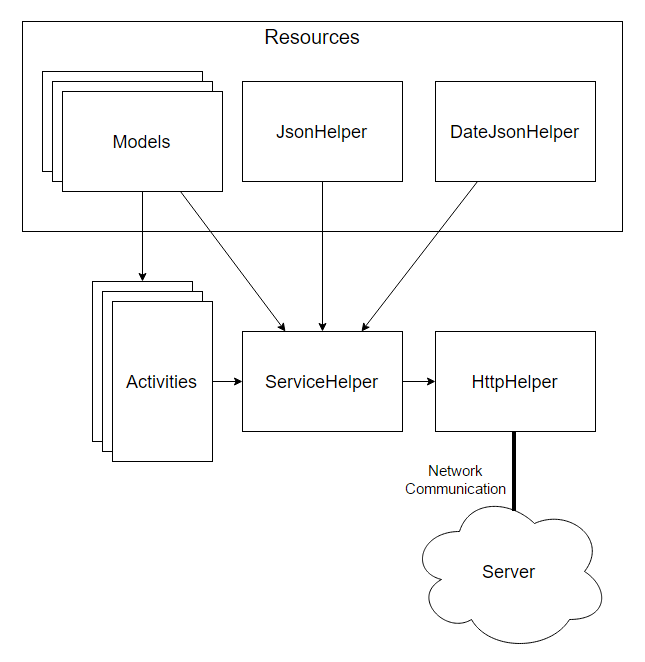
\includegraphics[width=\textwidth]{Pictures/application_dataflow.png}
	\caption{Processing data for server communication}
	\label{fig:application_dataflow}
\end{figure}